\section{Chords}

\subsection{Building chords}
In the previous sections we have learned about the major and minor scales. This information can be used to finally start to learn about chords.

\textbf{A major or minor chord is constructed by playing the 1st, 3rd and 5th note of a scale at the same time. That's it.}

\subsection{Open and barre chords}

When a chords is played that contains open strings, it is called an "open chord". When a chord is played without open strings, it is called a "barre chord".

The nice thing about barre chords is that you can move them up and down the neck. At that point the barre chord becomes more of a shape than a chord per se. Depending on what the root note is at a certain position, the barre chord will get a different name. We will see this later in the \textbf{CAGED system}.

On the next page in \autoref{fig:guitar_major_minor_chords} you will see all the major and minor chords listed. The chord \textbf{C} is a major chord and the chord \textbf{Cm} is a minor chords. The same holds for the other chords. Below each chords there are the 1st, 3rd and 5th notes from the respective scale (see \autoref{tab:guitar_natural_note_major_scale} and \autoref{tab:guitar_natural_note_minor_scale}).

The green dots indicate the root note. This is the note with the same name as the chord.

A couple things to note:

\begin{itemize}
	\item The root and the 5th note of a scale are same for both the major and minor variant.
	\item The 3rd note of minor chord is always a half step / 1 semitone lower than it is in the major chord.
\end{itemize}

The barre F chord is a good example of what was mentioned in the beginning. The thing about barre chords to become more like a shape that can become different chords. Compare the shape of the E and Em chords with the F and Fm chord shapes. Note how the shape is the same and there are no open strings in the F and Fm. By just moving the E chord shape a half step (one fret) to the right, the root note has changed and it is therefore now an F chord.

\newpage

\begin{figure}[h]
	\centering
	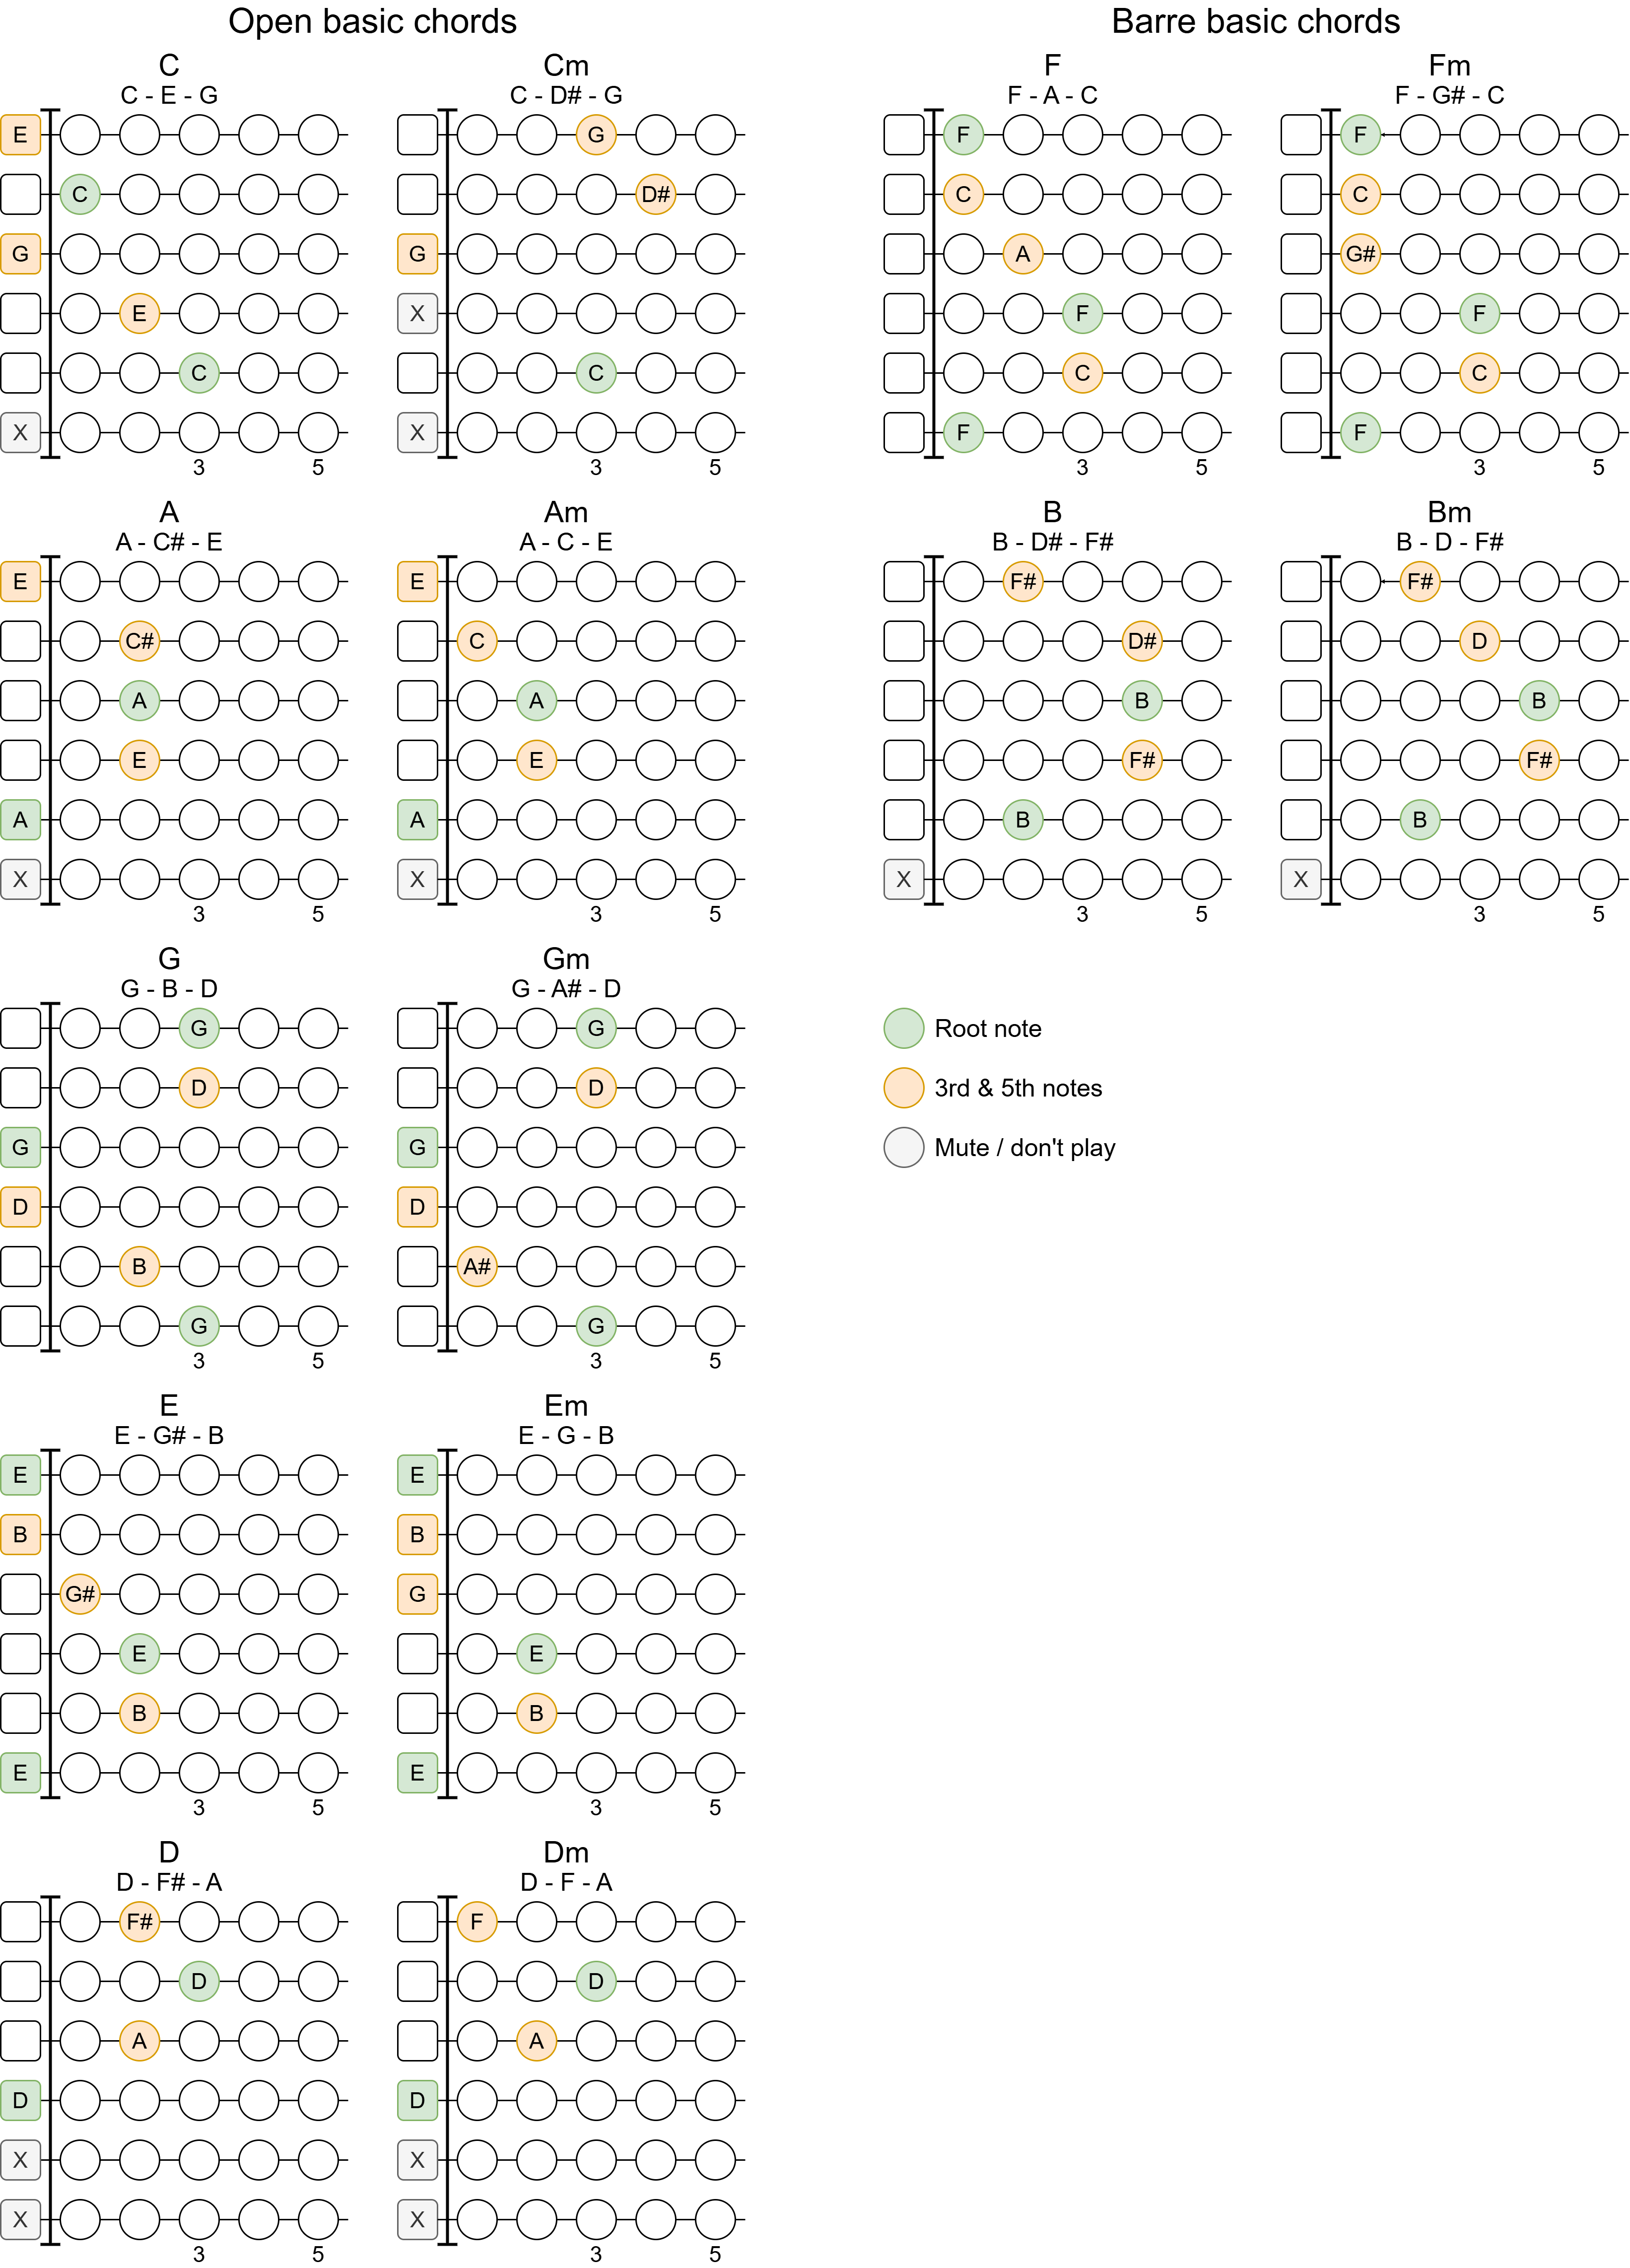
\includegraphics[height=0.9\textheight]{../../Images/GuitarBasicChords.png}
	\caption{Major and minor chords}
	\label{fig:guitar_major_minor_chords}
\end{figure}

\clearpage

Lets play some chords. The theme song (\autoref{fig:guitar_adventure_time}) of the Adventure Time series is a good start.

\begin{figure}[h]
	\centering
	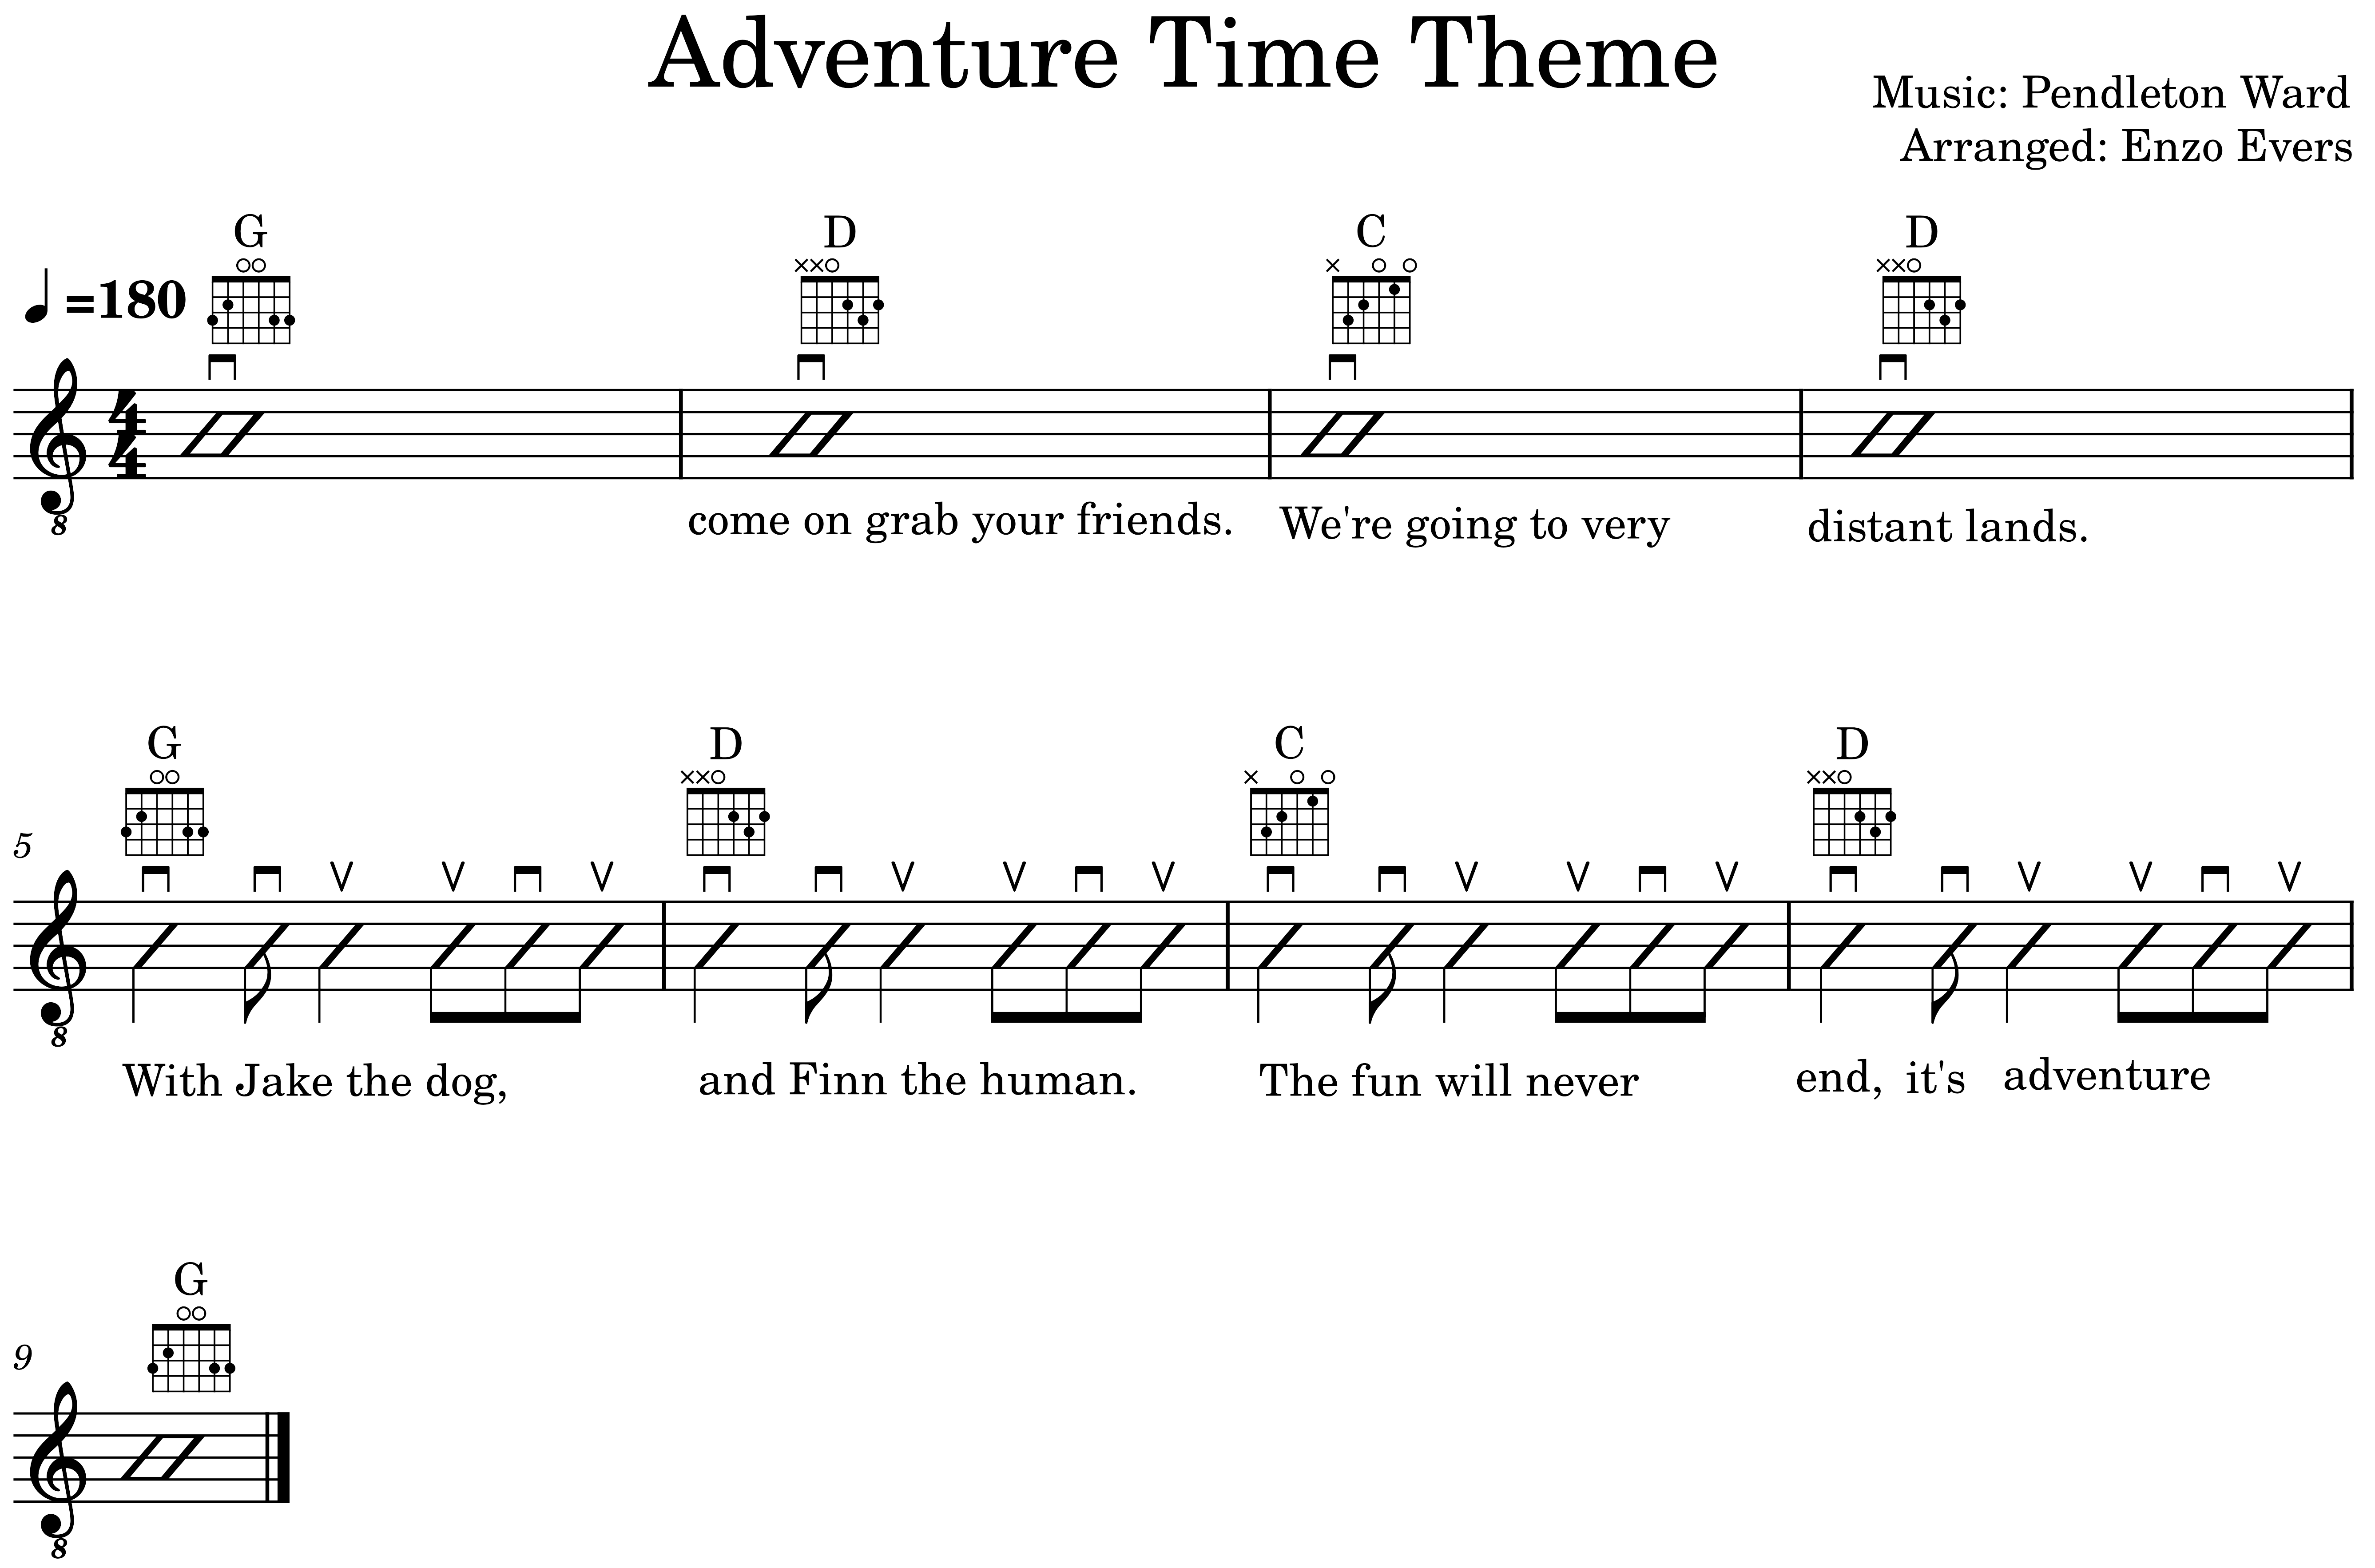
\includegraphics[width=\textwidth]{../../MuseScore/Guitar/GuitarAdventureTimeTheme.png}
	\caption{Adventure Time Theme Song}
	\label{fig:guitar_adventure_time}
\end{figure}